\section{Présentation du projet MARS} \label{sec:presentation_mars}

Le logiciel sur le quel j'ai été assigné se nomme MARS, qui est un acronyme signifiant \textit{Manage Alltech Resources
Simply}. Le but de ce programme, est donc de simplifier la gestion des resources, principalement des consultants,
plus facilement. Les utilisateurs sont donc assez réduit en nombre, vu qu'il s'adresse principalement à la direction
de Alltech, ce qui offre l'avantage de pouvoir facilement entrer en contact avec les clients en cas de modifications
non prévues, ou de besoin de précisions sur certain besoins.

\begin{figure}[H]
    \centering
    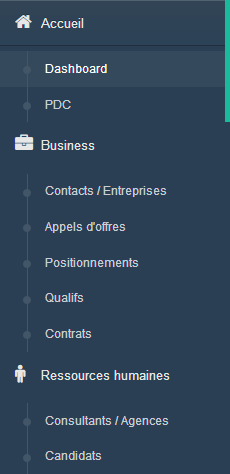
\includegraphics[width=.4\linewidth]{images/MARS/navbar.png}
    \caption{Barre de navigation de MARS} \label{fig:mars_navbar}
\end{figure}

Comme on peut le voir sur la figure \ref{fig:mars_navbar}, le site offre la possibilité de gérer plusieurs aspects
de l'entreprise comme les consultants, les différentes appels d'offres, et autres éléments liés à ces appels d'offres.
Un positionnement représente un premier contact entre une entreprise (via un appel d'offre) et un consultant. La page
positionnement sert alors à lier un consultant avec une entreprise. Une qualification est en quelque sorte une 
évolution d'un positionnement et représente un entretien entre un consultant et l'entreprise en vue d'un potentiel
contrat. Une qualification peut alors être dans plusieurs états :
\begin{itemize}
    \item [En Cours] Le consultant est en attente d'une réponse suite à son entretien.
    \item [Perdu] L'entreprise à répondu négativement sutie à l'entretien.
    \item [Stand By] L'entretien est en attente pour quelconque raison.
    \item [Abandonné] Ce qui veut dire que l'entretien n'aura potentielement pas lieu.
    \item [Gagné] L'entreprise à répondu positivement sutie à l'entretien, et le consultant peut alors effectuer un 
        contrat chez eux.
\end{itemize}